%===============================================================================
% $Id: ifacconf.tex 19 2011-10-27 09:32:13Z jpuente $  
% Template for IFAC meeting papers
% Copyright (c) 2007-2008 International Federation of Automatic Control
%===============================================================================
\documentclass{ifacconf}

\usepackage{graphicx,times}
\usepackage{natbib}        % required for bibliography
\usepackage{xcolor}

\usepackage[utf8x]{inputenc}
\usepackage{lmodern,textcomp}
\usepackage{multirow}
%\usepackage{subfig}
%\usepackage{caption}
\usepackage{tipa}
\usepackage{graphicx}
\usepackage{hyperref}
\usepackage{multirow}
\usepackage{verbatim}
\usepackage{booktabs}
\usepackage{booktabs,siunitx}
\usepackage{amsmath}
\usepackage{amsfonts}  
\usepackage{enumitem}

%===============================================================================
\begin{document}
\begin{frontmatter}

\title{Stochastic modelled grid outage effect on a solar home} 
% Title, preferably not more than 10 words.

\author[First]{Jesse-James PRINCE AGBODJAN}
\author[First]{Pierre HAESSIG} 
\author[First]{Romain BOURDAIS}
\author[First]{Herve GUEGUEN}

\address[First]{CentraleSupelec CNRS IETR (Institut d'Electronique et de Telecommunications de Rennes), UMR 6164, F-35000 Rennes, France (e-mails : \{jesse-james.prince-agbodjan, pierre.haessig, romain.bourdais, herve.gueguen\}@centralesupelec.fr)}

\begin{abstract}                % Abstract of not more than 250 words.
This paper focus on improving the notion of resilience of existing controllers based on Model Predictive control. The controller resulting that we have called \textit{resilient open loop feedback controller} takes into consideration a stochastic model of the grid during the design phase. Two stochastic grid outages model are considered. The new resileint OLFC is compared to the previous Resilient Model Predictive Controller and the results show that the former, closer to the reality exhibits the same behavior as the latter.
\end{abstract}
\begin{keyword}
Home Energy Management System (HEMS) , Resilience, Model Predictive Control (MPC), multi objectives optimization, Open Loop Feedback Controller(OLFC)].
\end{keyword}

\end{frontmatter}
%===============================================================================

\section{Introduction}
Home Energy Management System are based on controllers that optimize some economic criteria. This optimization is mainly done through balancing the grid, the renewable energy sources and the local storage, but the latter can also be utilize to enhance the energy independence and the resilience of the system when the grid fails. The importance of a grid failing might not be obvious but related works (CEER) showed that grid power outages habitually occur in off grid locations, less frequently in developed countries but when they do happen, they greatly impact people's live.

Of course it is arguable that the resilience during the outage depends on several parameters but one of the most influential is the quantity of energy in the storage when the failure appears. 

There is a lot of works on HEMS in general but a few deals with the behavior of the controller before and during an outage. Among them, \cite{HGhRBo2015,RRoFBe2014} propose reducing the user's comfort by shutting down a part of the demand as soon as the outage happens. That same idea is used in \cite{JMaHJa2016}, but an additional condition is to reserve at all time, a fixed quantity of energy storage to be used only in case of outage. In our previous work (\cite{JPrPHa2019}) the so called resilient model predictive controller uses the power of Model Predictive Control framework to dynamically choose the right level of energy within the storage when the failure happens and the part of the demand to shut down in order to increase the system resiliency.

The common thread between all the previous cited works is that they consider a deterministic model of the grid power outage i.e. one either clearly knows when the failure might happen (scheduled grid power outage) or not (unscheduled grid power outage). 

This work on the other hand, a direct extension of what we have proposed in \cite{JPrPHa2019}, is different in his character of considering a stochastic model of the grid behavior that is take into account during the design phase of the controller. What result is what we have called the Resilient Open Loop Feedback controller (OLFC) which according to the probability of occurrence of an grid outage which we get from the modelling, adapt his behavior.

The paper is further organized as follows. Section \ref{CaseStudy} describes briefly the main components of the system considered. Following in section \ref{ModelGriBeh} we propose two ways of modelling the grid behavior. In section \ref{Prob_Statement} we present the problem we are facing by stating the objectives of the controller and introduce the results obtained in the previous sections into the design of the OLFC in section \ref{OLFC}. The next section presents the results and some analysis of the different simulations. Conclusion and future directions are given at the end in section~\ref{conclusion}.

%%
\section{Case Study}\label{CaseStudy}
\begin{figure}[!ht]
        \begin{center}
                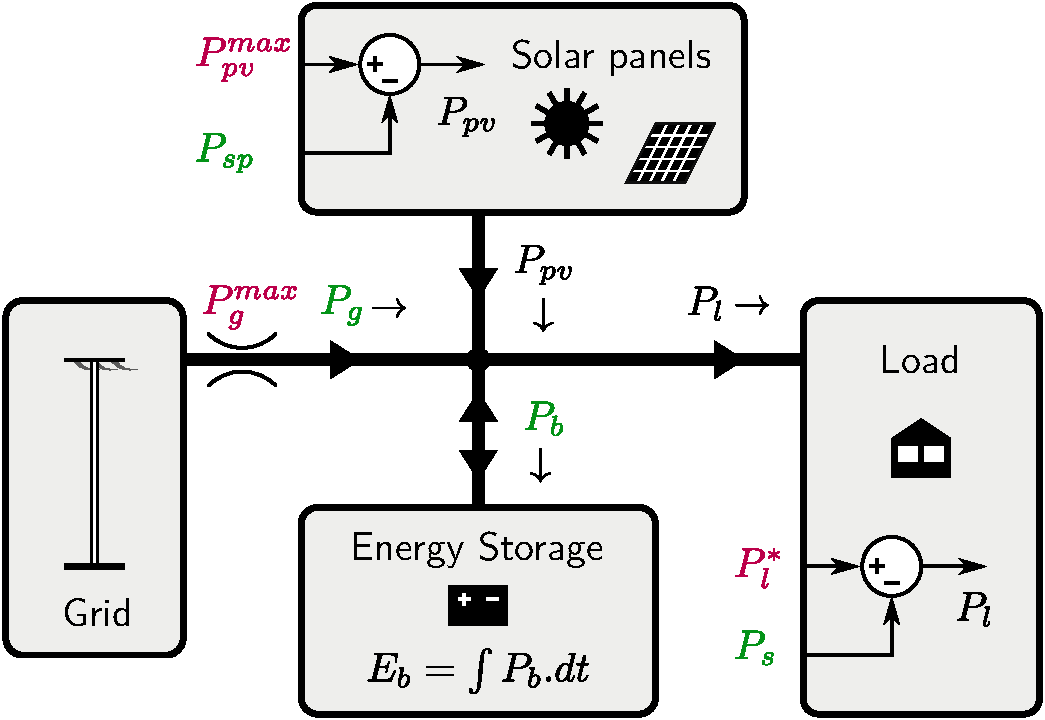
\includegraphics[width=0.9\columnwidth]{Figures/solar_home_compact.pdf}
        \end{center}

        \caption{Power flow model of a solar home.
        The decision/controlled variables are colored in green, external data are colored in red (Solar potential and desired consumption), internal variables are colored in black.
        }
        \label{fig:solhome}
\end{figure}
\quad The Case Study is a solar home represented by its power flow model (Fig.~\ref{fig:solhome}). It is a discrete time model of a photovoltaic system with storage for the auto-consumption of a residential consumer connected to the electrical grid. It is comprised of 2 externals known variables $P_{pv}^{max}$, $P_l^*$ respectively the solar potential production  and the power demand of the house (in red) and 4 controlled variables $P_g$, $P_{sp}$, $P_b$ and $P_s$ (in green) defined as follow : 
\begin{itemize}
\item $P_g$ is the power drawn from the grid bounded bellow and above
respectively by 0 (selling energy is not authorized) and the maximum power subscribed by the user $P_g^{max}$,
\item $P_{sp}$ is the spilled solar power when it cannot be used directly or stored, therefore $P_{pv}$ the actual solar energy used in the system is the difference between $P_{pv}^{max}$ and $P_{sp}$, $P_{pv} = P_{pv}^{max}-P_{sp}$
\item $P_s$ the shedded power representing the energy not provided to the load (house), hence the actual power provided to the load $P_l = P_l^* - P_s$
\item $P_b$ the power into/out of the storage unit, which accumulation over time gives the energy in the battery $E_b$, of course constrained above by $E_b^{max}$ the maximum capacity of the battery. 
\end{itemize}

\section {Model of the grid behavior}\label{ModelGriBeh}
 In this paper we are mainly interested in the behavior of the controller before an outage appears. To do so, the availability an non availability of the electricity grid must be modelled.  Two frameworks which are the Bernoulli process  and the Markov Chain (MC)(\cite{RBiRna1992}) are used to reach that objective.
 \subsection{Bernoulli process model of the electrical grid}
 The Bernoulli process (BP) is a finite sequence of identically distributed and independent (iid) r.v that can only takes two values. The probability mass function of the r.v  $P_g^{max}$ representing the state of the  grid is then given by :
  \begin{itemize}
\item $\mathbb{P}(P_g^{max} = P_0) = \lambda $
\item $\mathbb{P}(P_g^{max} = P_1)= 1-\lambda $ 
\end{itemize}
At each instant $k$, the probability of the grid being unavailable and available respectively are therefore given by $\lambda$ and $ 1-\lambda$

\subsection{Markov Chain model of the electrical grid }
 We modeled the grid secondly by a two states Markov chain given by fig. \ref{fig:MarChain} where $\lambda$ is said to be the $failure \; rate$ while $\mu$ is the $repair\; rate$.
 \begin{figure}[!ht]
        \begin{center}
                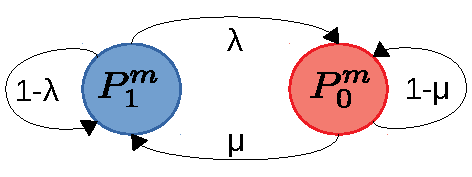
\includegraphics[width=0.60\columnwidth]{Figures/MarChain_paper.pdf}
        \end{center}
        \caption{Markov chain model of the electrical grid}
        \label{fig:MarChain}
\end{figure}
Consider that the process modelled by the different states of the electrical grid takes either the value $P_1$ when the grid is available or $P_0$ when the grid is unavailable. Let's $P^{max}_{g,k}$ denote its value at time period $k$. It follows that if $P_{g,k}^{max} = P_0$ or $P_{g,k}^{max} = P_1$ respectively the process is said to be in state unavailable and available at time $k$. Whenever the process is in some state, there is a fixed probability that it will be next in the other state or remain in the same. That is : 
\begin{subequations}\label{eq:MarChain}
\begin{align}
    \mathbb{P} \lbrace P^{max}_{g,k+1} =  P_0 | P^{max}_{g,k} = P_1, \ldots, X_0 \rbrace  &= \lambda, \\
    \mathbb{P} \lbrace P^{max}_{g,k+1} =  P_1 | P^{max}_{g,k} = P_1, \ldots, X_0 \rbrace  &= 1-\lambda, \\
    \mathbb{P} \lbrace P^{max}_{g,k+1} =  P_1 | P^{max}_{g,k} = P_0, \ldots, X_0 \rbrace  &= \mu, \\
    \mathbb{P} \lbrace P^{max}_{g,k+1} =  P_0 | P^{max}_{g,k } = P_0, \ldots, X_0 \rbrace  &= 1-\mu,
\end{align}
\end{subequations}

where, $X_0$, $P^{max}_{g,k}$ and $P^{max}_{g,k+1}$ represent respectively all the past states that the process has visited, the present and the future state. 

Equation (\ref{eq:MarChain}) states that, for the MC represented in Fig. \ref{fig:MarChain}, the conditional distribution of any future state $P^{max}_{g,k+1}$ given all the past states resumed in $X_0$ and the present state $P^{max}_{g,k}$ is independent of the past states and
depends only on the present state. The one step transition probabilities matrix representing the MC is then given by: 
\begin{equation}\label{eq:MarChain_TransMat}
\mathbf{T} = 
  \begin{bmatrix}
 1-\lambda  & \lambda \\ 
 \mu & 1- \mu
\end{bmatrix} . 
\end{equation}

Let's denote by $\Pi^n$ the n-step transition probability vector of the process. The \textit{Chapman–Kolmogorov equations} provide a method for computing this n-step  transition probability vector such that: 
\begin{subequations}
    \begin{align}
    \Pi^n & = \Pi^0 \, \mathbf{T}^n, \quad \forall n \geq 1 \label{eq:nsStaVec1} \\
          & = \bigl[ \underbrace{\mathbb{P} (P_g^{max} = P_1 | \Pi^0)}_{\pi^n_1}\quad \underbrace{\mathbb{P} (P_g^{max} = P_0 | \Pi^0)}_{\pi_{0}^n} \bigl] \label{eq:nsStaVec2},
\end{align}
\end{subequations}
where the first and the second column of equation (\ref{eq:nsStaVec2}) represent respectively the probability of the grid being available ($\pi_{1}^n$) or unavailable ($\pi_{0}^n$) at time $n$ given that the initial (present) state probability vector  is $\Pi^0$. At the present state we know if the electrical grid is available or not, hence $\Pi^0$ taking either the value [1 0] when the grid is available and [0 1] on the contrary.

It is important, to emphasis here that $\pi^n_0$ and $\pi^n_1$ correspond respectively to $\mathbb{P}(P^{max}_g = P_0)$ and $\mathbb{P}(P^{max}_g = P_1)$ or equivalently $\lambda$ and $1-\lambda$  in the Bernoulli model.

\section{Problem statement}\label{Prob_Statement}
For the solar home, the controller defines two objectives :
\begin{itemize}
    \item ObjA: Minimizing the electricity bill given by $C_gP_g$, where $C_g$ is the electricity price
    \item ObjB: Minimizing the  discomfort bill given by $C_sP_s$, where $C_s$ is a virtual price associated with a unit of discomfort
\end{itemize}
The multi-objectives problem A and B are converted into a single objective optimization problem through linear scalarization (\cite{Deb2014}) where the objectives A and B are aggregated with positive weights which serve to normalize the main cost functions as well as organize the sub-objectives function
priority. Since the price of the electricity (the weight associated with ObjA) is a problem input, our only degree of freedom is the weight associated with ObjB ($C_s)$ that we choose to be higher than that of ObjA, i.e. $C_s \gg max(C_g)$ to transcribe the fact that avoiding the discomfort is more important than paying a lower electricity bill. Note that the electricity price can vary during the day.

The problem to be solved is therefore completely  described by:
\begin{align} 
& \underset{P_g,P_{sp},P_b,P_s}{\text{min}} J = \sum_{k=1}^{N} C_gP_g + C_sP_s \label{eq:cost2min}\\
& \text{\hspace{20px} s.t.\hspace{15px}} 0 \leq P_g\leq P_g^{max} \label{eq:Pgr_cons} \\
& \hspace{52px} 0 \leq P_{sp} \leq P_{pv}^{max} \label{eq:Pcu_cons}\\
& \hspace{52px} 0 \leq P_s \leq P_l^* \label{eq:Psh_cons} \\
& \hspace{52px} 0 \leq E_b \leq E_b^{max} \label{eq:Est_cons} \\
& \hspace{52px} E_b(k+1) = E_b(k) + P_b(k)\Delta_t \label{eq:Est_dyn}  \\
& \hspace{52px} P_g- P_b+ \underbrace{P_{pv}^{max}-P_{sp}}_{P_{pv}} =\underbrace{P_l^* - P_s}_{P_l} \label{eq:Engy_csvt} 
\end{align}

Note that all the variables and constraints of the previous problem are evaluated at each instant $k \in \{1, \ldots, N \}$, i.e. should therefore been indexed by `` $k$ '' but we have deliberately choose not to  put it for clarity and simplicity sake as we will do for the rest of the paper.

Introduced in the model Predictive Control (MPC) framework, the previous problem is no longer solved over the long horizon N but rather on a sliding horizon H. It becomes : 
\begin{equation}\label{eq:MPCsys}
\left. 
\begin{aligned}
&\underset{P_g,P_{sp},P_b,P_s}{\hspace{10px} \text{min} \hspace{10px}J_H =} \sum_{j=k}^{k+H} C_gP_g + C_sP_s\\
& \text{\hspace{20px} s.t.\hspace{15px}} (\ref{eq:Pgr_cons}),(\ref{eq:Pcu_cons}),(\ref{eq:Psh_cons}), (\ref{eq:Est_cons}), (\ref{eq:Est_dyn}),(\ref{eq:Engy_csvt})
\end{aligned}\right \}
\end{equation}

If the trajectory of all the problem's inputs i.e. $P_l^*$, $P_{pv}^{max}  \text{ and } P_g^{max}$ are known in advance, solving it is straight because we obtain a deterministic optimization problem. 
That is the case that have been treated in \cite{JPrPHa2019}.

In the other hand consider now the case where $P_g^{max}$ is a random variable (r.v) taking its value in a set $\mathcal{P}$ defined as $ \mathcal{P} = \left \{ P_0 , P_1\right \}$. Note that $P_0=0$ and $P_1$ is the maximum power subscribed by the user. More Explicitly if the r.v : \begin{itemize}
\item $P_g^{max} = P_0 \rightarrow$ the grid is not available, an outage is occurring ; 
\item $P_g^{max} = P_1 \rightarrow$ the grid is available and we can draw energy from it . 
\end{itemize}

Taking now into consideration the stochastic characteristic of $P_g^{max}$, problem (\ref{eq:MPCsys}) is ill defined since we do not have a clear definition of what constraint (2.a) means. Yet, such a definition ought to be found if we want to solve the said problem. Two optimization fields  provide a framework which give a sensible meaning to such a ``random inequality system”. These are Robust Optimization (RO) (\cite{BenTal2009}) and Probabilistic Programming (\cite{Ankopa1995}).

The \textit{worst-case-oriented} RO approach as its name indicates, to solve this problem would consider the value of the r.v. (i.e. $P_0$) that produces the worst objective cost value. This results is of course a valid robust sub-optimal solution to the problem at each instant but is not interesting to be implemented since in other words it means considering that the grid is never available which is spurious.
 
 Probabilistic Programming problem can be formulated using two different approaches, the $probabilistic\,/\,chance$  $constraint (CC)$ and  the multistage stochastic optimization.
  
 CC has been first introduced by \cite{AChWCo1958} and further developed in \cite{AChWCo1959,AChWCo1962,AchWCo1963}. The field received later on several contribution among which \cite{AnPre1970,Tsentai1988,APrBVi1998,RHenrion2002,RHenrion2007}. 
 Chance constraint programming deal with constraints of the form
 \begin{equation}\label{eq:CCnomform}
     \mathbb{P}[g(x,\xi)\geq 0]\geq p,
 \end{equation}
 where $x \in \mathbb{R}^n$ is the decision vector, $\xi \in \mathbb{R}^m$ a r.v. and  $g: \mathbb{R}^n \mathsf{\,x\,}\mathbb{R}^m \rightarrow \mathbb{R}^k$ a constraint mapping. The level $p \in (0,1)$ is user defined and represent the safety for the decision $x$. In other words, the constraint \eqref{eq:CCnomform} says that we wish to take a decision $x$ that satisfies the k-dimensional random inequality system $g(x,\xi)\geq 0 $ with high enough probability. An important case of constraint \eqref{eq:CCnomform} is where  $x$ and $\xi$ are not coupled through the mapping but appear separate. In this case, $g$ is then of the form $g(x,\xi) = h(x)− \widetilde{g}(\xi)$. The constraint \eqref{eq:CCnomform} can then be rewrite as:
 \begin{align}
     G(x)&:= \mathbb{P}[h(x) \geq \widetilde{g}(\xi)]\geq p \label{eq:Gdex_eq1}\\
         &:= F_\xi{h(x)}\geq p \label{eq:Gdex_eq2}
 \end{align}
 and is referred to as separable chance constraints. Note that \eqref{eq:Gdex_eq2} is \;\; obtained \; by \; considering  \;that \; $\widetilde{g} = \xi$ and \\  $\mathbb{P}[\xi \leq h(x)] = F_\xi(h(x))$, where $F$ is the $ cumulative$  $distribution function$ of $\xi$.
 When using chance constraint, an important fact is that the r.v  is assumed to have a normal law. In our case we are in the presence of a r.v variable which have a binary (Bernoulli) distribution which are not applicable.

 The  multistage stochastic optimization  introduced in [ref] consider all the possible realizations of a r.v.  at each stage and resolve an unique optimization problems accordingly. The size of the resulting problem grows exponentially in consonance with the distribution of the r.v. and the number of stages considered. For instance take the r.v in our case which can assume two values at each instant for a MPC horizon of 24 hours  with a command frequency of 30 minutes, the problem has $2^{48}= 281.474.976.710.656 \approx 2.10^{14}$ variables.
 
 \section{The open loop feedback controller (OLFC)}\label{OLFC}
\begin{table*}[!htbp]
%% increase table row spacing, adjust to taste
\renewcommand{\arraystretch}{1}
\caption{Controller Performances for both Low and High failure rate}
\noindent
\centering
  \begin{minipage}{\linewidth} %Use the minipage environment to footnote tables
 
        \begin{center}
            \begin{tabular}{c||*{4}{c|}c||*{4}{c|}c||}
		\cline{2-11}
	
	 &\multicolumn{5}{c||}{\textbf{No outage}} & \multicolumn{5}{c}{\textbf{With outage}} \\ \cline{2-11}
	
	
	  &\multirow{2}{*}{$E_{g}$} & \multirow{2}{*}{$E_{s}$}
	& \multicolumn{3}{c||}{\begin{tabular}[c]{@{}c@{}}$E_b$\end{tabular}} &\multirow{2}{*}{$E_{g}$}  &\multirow{2}{*}{$E_{s}$} &\multicolumn{3}{c||}{\begin{tabular}[c]{@{}c@{}}$E_b$\end{tabular}}\\ \cline{1-1}\cline{4-6}  \cline{9-11} 
	
	 $\lambda$ &  &  &Beg &Mid  &End &   &   &Beg   &Mid   &End \\\cmidrule[1pt]{1-11}
	 Low  &19.3   &0   &0  &0.2   &0   &4.7  &14.6  &0    &0.2    &0 \\ \cline{1-1}
	 High &26.7   &0   &0  &4.5 &7.4 &9.0  &10.3  &0  &4.5  &0\\\cmidrule[1pt]{1-11}
	        \end{tabular}
        \end{center} \label{tab:CompTable1}
    \end{minipage}
\end{table*}
Consider problem (\ref{eq:MPCsys}) which is the minimization of the cost $J_H$ over the horizon which span from $k$ to $k+H$. Let us subdivide that problem into two sub-problems which are the present and the future sub-problems. For the present sub-problem indexed by $k$, let us assume that the r.v. $P_g^{max}$ has revealed already. In this case, dispatching the energy in each branch of the system is simple deterministic problem. 
Now consider the future sub-problem indexed by $k+1$ that is we need to choose how much energy must be drawn from the grid before we know if the latter is available or not. Similar problems can be found in the literature under the name Newsvendor/Newsboy Inventory Problem [ref or not]. We are in the stochastic programming here and now framework. 

Mathematically here is how our future sub-problem describes. Recall constraint (\ref{eq:Pgr_cons}), that we can rewrite as the set of 2 others constraints as follows,
\begin{subequations}
    \begin{align}
        0 &\leq P_g(k+1) \label{LhsPg}, \\
        P_g(k+1) &\leq P_g^{max}. \label{RhsPg}
    \end{align}
\end{subequations}
Taking into account that the lower bound of the r.v. $P_g^{max}$ equals the right hand side of (\ref{LhsPg}), it follows that no matter the value that the r.v. takes on in the future, constraint  (\ref{LhsPg})  is always satisfied. Consider now the random constraint (\ref{RhsPg}) that we rewrite in its deterministic form as follows :
\begin{subequations}
    \begin{align}
        P_g (k+1) &\leq P_1 \label{Rhs1}\\
        P_g (k+1) & \leq P_0 \label{Rhs2}
    \end{align}
\end{subequations}
Since $P_1$ is a upper bound 
Suppose that after being solved the future sub-problem result for the future problem gives a $P_g$ such that $P_0< $

 
 Constraints (2.b) is now replaced by two constraints as follows
 
 \begin{align}
 P_g &\leq P_1 \label{NewCons1}\\
 P_g - P_{ex} & \leq P_0 \label{NewCons2}\\
 P_{ex} & \geq \label{NewCons3}0 
 \end{align}
$P_{ex}$ can be considered as an external source of energy that will be  only used as last resort when the grid fails in the future. To do so its usage must be minimize hence we add the cost $C_{ex}P_{ex}$ in the previous optimization cost as follows: 
\begin{equation}
    J_{OLFC} = J_H + \sum_{j=k+1}^{k+H} P_{ex}(j)C_{ex}(j),
\end{equation}
where $C_{ex}$ the cost of using the external source is the same as the cost of shedding some energy i.e $C_{ex} = C_s$. Note  now that all the values of $C_g$ and $C_{ex}$ from $k+1$ to $k+H$ are all random since they depends on the realisation of the r.v. $P_{g}^{max}$ at those time. It follows that instead of minimizing the new cost function $J_{OLFC}$, we are going to minimize it's expectation as follows:
\begin{equation}
    \begin{split}
        \mathbb{E}[J_{OLFC}] &= \mathbb{E}[J_H + \sum_{j=k+1}^{k+H}C_{ex}P_{ex}] \\
                             &=  C_g(k)P_g(k) + C_sP_s(k) \\
                             &\hspace{12px}+\sum_{j=k+1}^{k+H}  C_sP_s(j) + \pi_{\;\,1}^{j-k}C_g(j)P_g(j)\\
                             &\hspace{85px} + \pi_{\;\,0}^{j-k}C_{ex}P_{ex}(j). 
    \end{split}
\end{equation}

The complete problem solved by OLFC is therefore given by: 

\begin{equation}\label{eq:OLFCsys}
\left. 
\begin{aligned}
&\underset{P_g,P_{sp},P_b,P_s,P_{ex}}{\hspace{10px} \text{min} \hspace{10px}\mathbb{E}[J_{OLFC}]}\\
& \text{\hspace{20px} s.t.\hspace{15px}}(\ref{eq:Pcu_cons}),(\ref{eq:Psh_cons}),(\ref{eq:Est_cons}),(\ref{eq:Est_dyn}),(\ref{eq:Engy_csvt}),(\ref{NewCons1}),(\ref{NewCons2}),(\ref{NewCons3})
\end{aligned}\right \}
\end{equation}



 \section{Simulation and results}
 
 
 \subsection{Simulation settings}
 All of our simulations have been done using \href{http://www.juliaopt.org/}{Julia} a high-level, high-performance dynamic programming language for technical computing with the \href{https://www.mosek.com/}{Mosek} toolbox. 
 
 Our simulations use a data extracted from ``\href{https://www.ausgrid.com.au/Common/About-us/Corporate-information/Data-to-share/Solar-home-electricity-data.aspx}{Solar home electricity data}'', a dataset of the Australian electricity distribution company Ausgrid. The dataset comprises of the home consumption ($P_l^*$) of several users and the solar potential ($P^{max}_{pv}$) recorded at the frequency of 30 minutes. The simulation is carried over three successive days chose randomly. We suppose that the grid failure occurs at 12:00 a.m right at the beginning the second day (denoted by a red doted vertical line on Fig.\ref{fig:LOwFailYesOut}, \ref{fig:HighFailYesOut} and remains until the end of the simulation. A whole day (H= 48 i.e. 24h) is considered as prediction horizon and $C_{g}$ consist of two energy price defined as follow : 
\begin{itemize}
 \item $C_{night}$ : Off-peak hour, from 12:00 a.m. to 6:00 a.m (highlighted in light blue on Fig. \ref{fig:LOwFailNoOut}, \ref{fig:HighFailNoOut}, \ref{fig:LOwFailYesOut}, \ref{fig:HighFailYesOut})
 \item $C_{day}$ : peak hour from 6:30 a.m. to 23:30 p.m
\end{itemize}

 
 \subsection{Simulation results and analysis}
 
 \begin{figure*}[!ht]
  
    \begin{minipage}{.49\linewidth}
       
        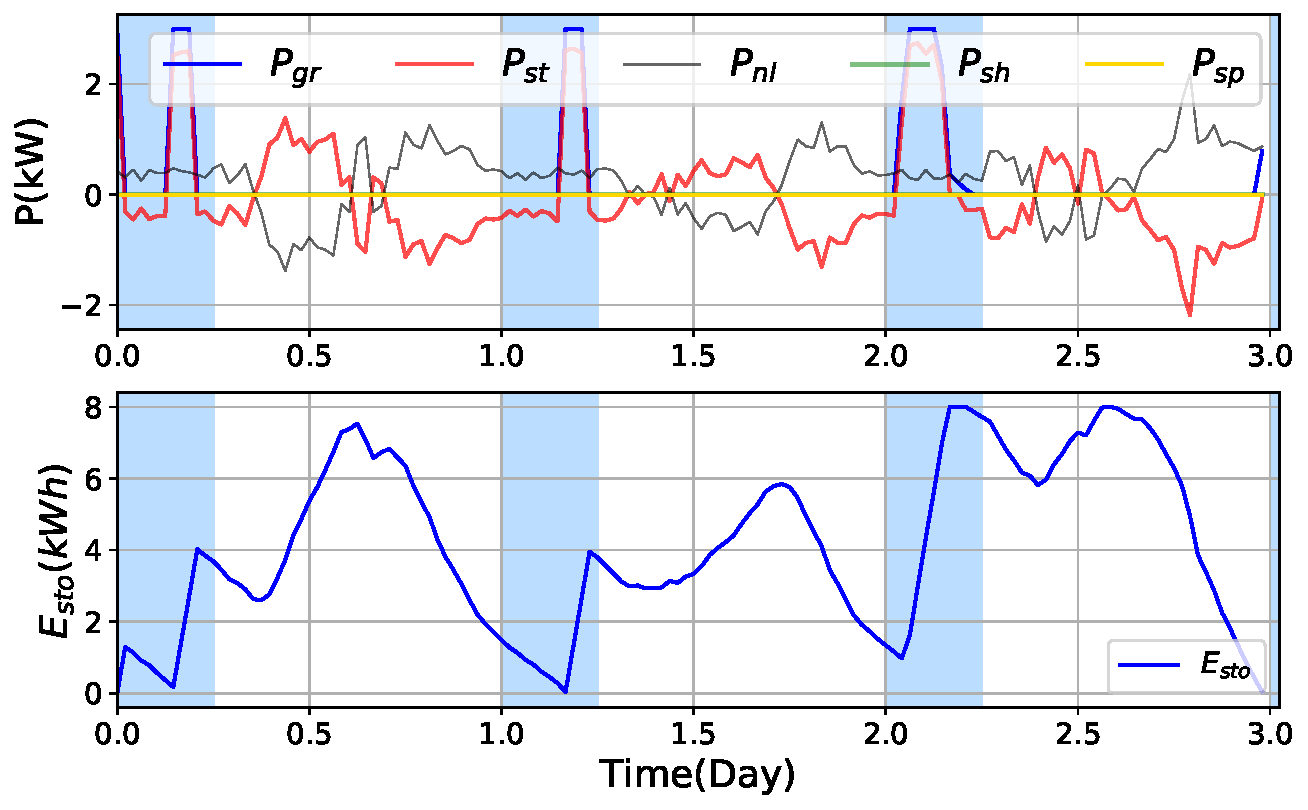
\includegraphics[height=2.5in,width=1\columnwidth]{Figures/Mc_LowFailNoOut.pdf}
        \caption{Low prob of failure, No outage}
        \label{fig:LOwFailNoOut}    
    \end{minipage}%
    \begin{minipage}{.01\linewidth}
      \hspace{1px}
    \end{minipage}%
    \begin{minipage}{0.49\linewidth}
        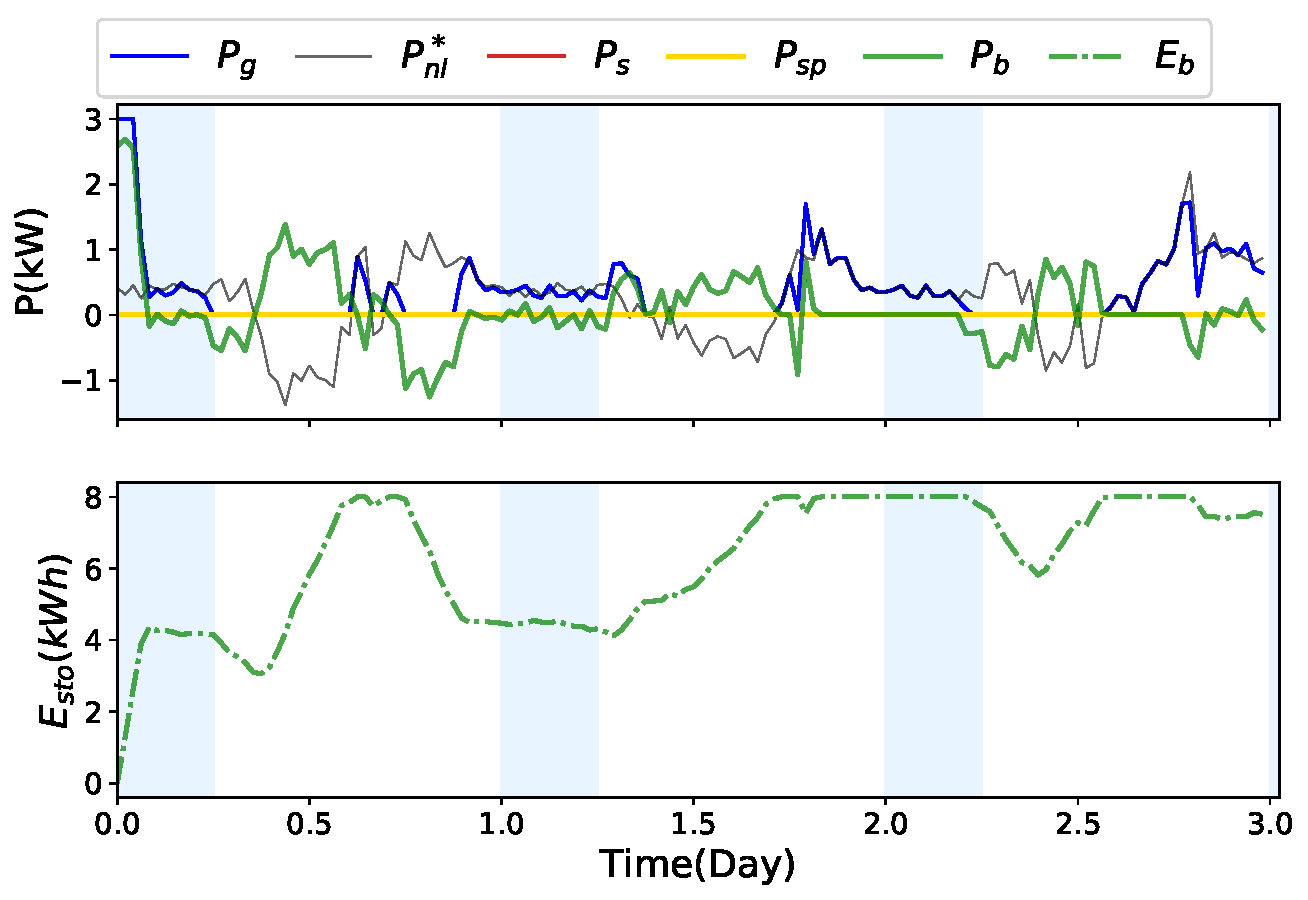
\includegraphics[height=2.5in,width=1\columnwidth]{Figures/Mc_HighFailNoOut.pdf}
        \caption{High prob of failure, no outage}
        \label{fig:HighFailNoOut}
    \end{minipage}
\end{figure*}

\begin{figure*}[!ht]
    \begin{minipage}{.49\linewidth}
        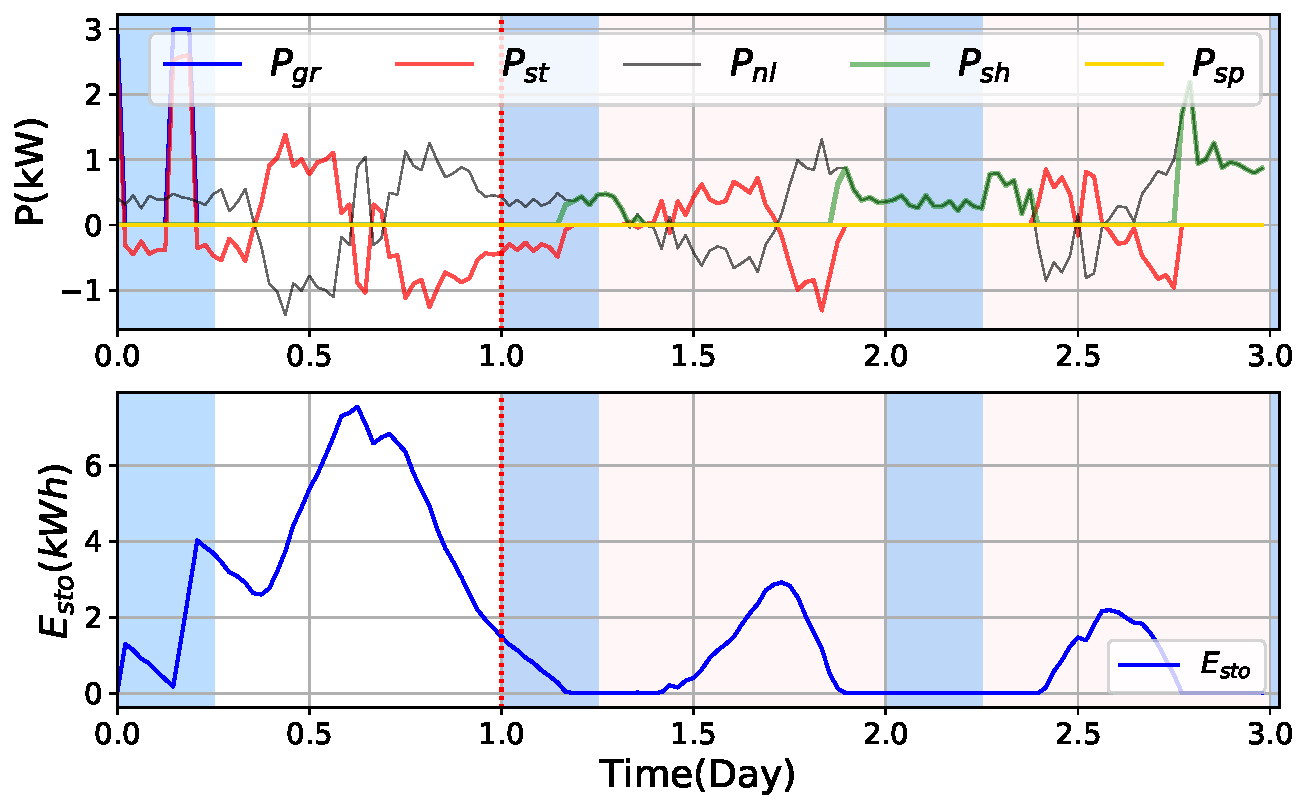
\includegraphics[height=2.5in,width=1\linewidth]{Figures/Mc_LowFailYesOut.pdf}
        \caption{Low prob of failure, with outage}
        \label{fig:LOwFailYesOut}    
    \end{minipage}%
    \begin{minipage}{.01\linewidth}
      \hspace{1px}
    \end{minipage}%
    \begin{minipage}{0.49\linewidth}
        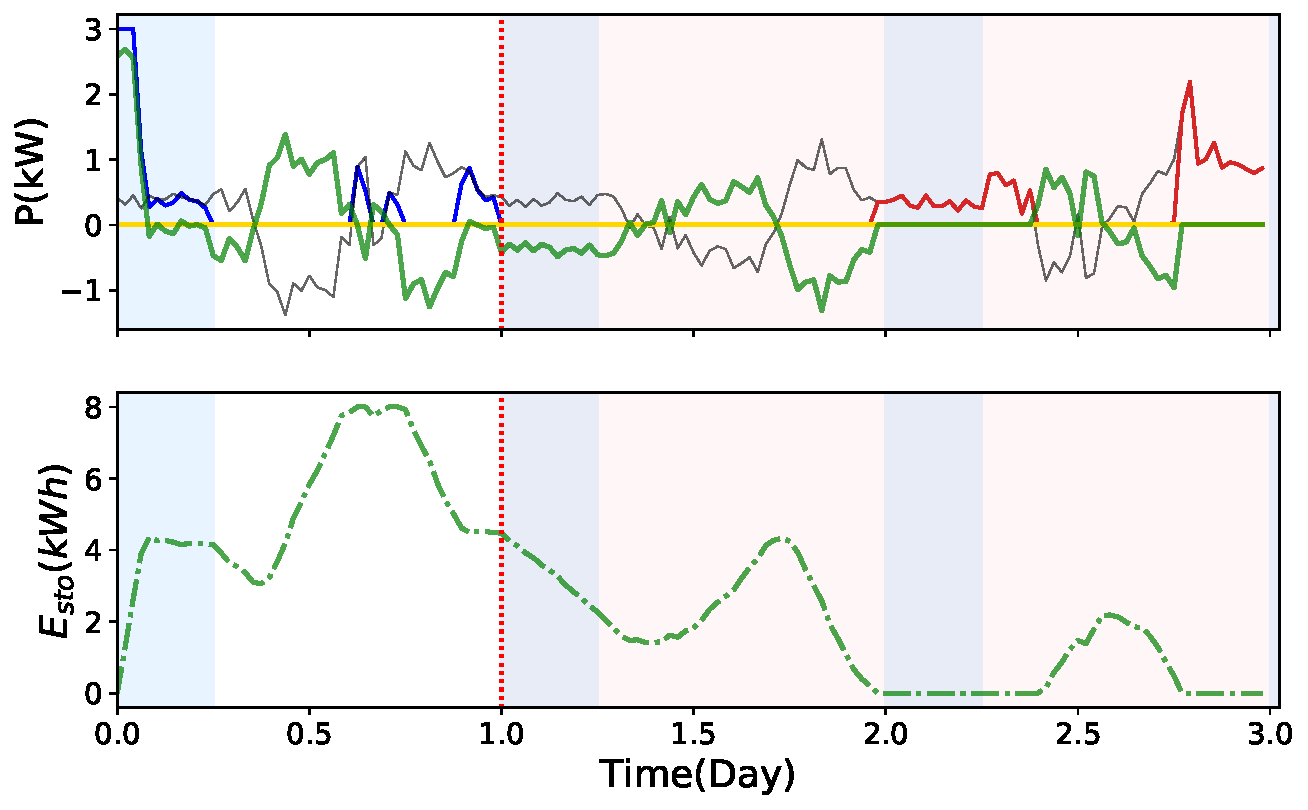
\includegraphics[height=2.5in,width=1\columnwidth]{Figures/Mc_HighFailYesOut.pdf} 
        \caption{High prob of failure, with outage}
        \label{fig:HighFailYesOut}
    \end{minipage}
\end{figure*}

 \begin{figure}[!htb]
        \begin{center}
                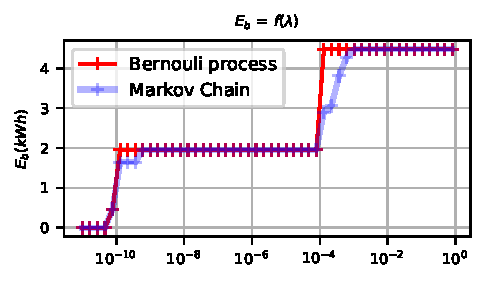
\includegraphics[width=0.9\columnwidth]{Figures/Mc_vs_Bp.pdf}
        \end{center}
                \vspace{-8px}

        \begin{center}
                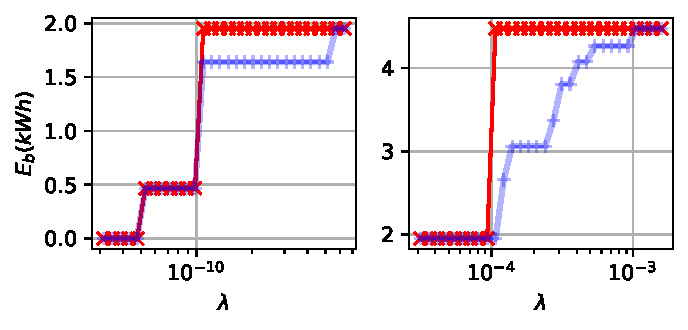
\includegraphics[width=.9\columnwidth]{Figures/Mc_vs_BpZoom.pdf}
        \end{center}
        \vspace{-8px}
        \caption{Comparison of the Energy inside the storage at the moment the outage occurs for the Bernoulli process and  Markov chain modeling of the grid behavior.
        }
        \label{fig:BernouVsMar}
\end{figure} 

\begin{figure}[!htb]
        \begin{center}
                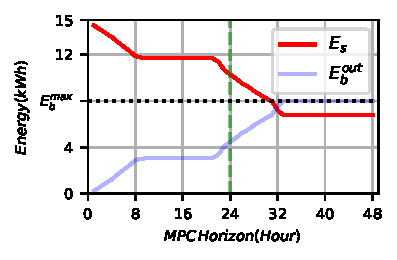
\includegraphics[width=.9\columnwidth]{Figures/MPCHorr.pdf}
        \end{center}
        \vspace{-8px}
        \caption{Evolution of $E_s$ and $E_b^{out}$ function of the MPC horizon.
        }
        \label{fig:Es&EbOut}
\end{figure} 
  For the set of simulations we have considered solely the MC's model of the grid behavior. It is the more realistic of both models since it encompass as well as the failure as the repair rate of the grid. We are mainly going to compare the behavior of the OLFC for a low and a high failure rate whether the outage actually happens or not. Fig. \ref{fig:LOwFailNoOut}, \ref{fig:HighFailNoOut} are associated with the case where the outage does not happen while Fig. \ref{fig:LOwFailYesOut}, \ref{fig:HighFailYesOut} are associated with the case where the outage does happen. The left and right figure respectively depicts the behavior with a low and high failure rate. 
  
  The higher sub-figures of each figure present the dynamic of  five electrical signal in the time. They are: the power drawn from the grid($P_g$), the energy not provided to the house ($P_s$), the wasted solar potential ($P_{sp}$), the power into the storage ($P_b$) defined all in section \ref{CaseStudy} and $P_{nl}$ which is the difference between the house demand and the solar potential i.e. $P_{nl} = P_l^* - P_{pv}^{max}$. Note that $P_{nl} < 0$ implies that there is enough solar potential to fully meet the household demand and to spare some energy into the battery. Oppositely $P_{nl} > 0$  indicates that the solar potential is not sufficient to satisfy on its own the house demand and therefore must be supplemented by the others sources. The lower sub-figures show the dynamic of the energy within the battery during the simulations. Table \ref{tab:CompTable1} present the numerical result associated with Fig.\ref{fig:LOwFailYesOut}, \ref{fig:LOwFailNoOut}, \ref{fig:HighFailYesOut}, \ref{fig:HighFailNoOut} 
  
  With a low failure rate, one observes that the OLFC only uses the grid during the night, especially during the off-peak hours when the electricity price is the lowest. With a high failure rate, besides on using  more of the grid during the off-peak hours (4.7kWh vs 6.5kWh) the strategy uses the grid also during the day to charge up the battery up to a certain point henceforth result in reducing the energy not provided to the house during the outage. Fig. \ref{fig:HighFailYesOut} shows that even with a high probability of failure, the OLFC from the beginning of the second day was no longer able to provided the house with its energy demand since there is no energy left inside the battery. A way to improve the strategy efficiency i.e to reduce even more the energy not provided is to prolong the MPC horizon. Fig. \ref{fig:Es&EbOut} show the evolution of the energy not provided to the load and the level of energy within the battery when the outage happens in function of the MPC horizon. The longer the horizon, the more energy is stored inside the battery until its maximum capacity is reached. Consequently the less is the energy not provided to the house when the outage happens.
  
  The next set of simulation have been done in order to compare the performances of both grid models. Since the quantity of energy within the battery at the instant the outage happens i.e. $E_b^{out}$ is an important factor that influence the energy not provided to the household during outages, we choose it to be the comparing factor. We therefore vary the failure rate $\lambda$ from a very low ($10^{-12}$) to a high ($10^{-0.01}$) probability for both grid models (maintaining throughout the simulation a constant repair rate $\mu=0.1$ that we have chose empirically in the case of the Markov chain's) and recorded for each value the corresponding $E_b^{out}$.
  
 On the higher subplot, Fig. \ref{fig:BernouVsMar} shows the result we have obtain for that variation while the lower subplots are a zoom on the left and right side of the higher image. There are three main failure rate \textcolor{red}{range/levels} that can be distinguish i.e. $(-\infty,10^{-10}[$, $(10^{-10},10^{-4}[$, $(10^{-4},0.99)$. When considering the first two, both grid models seems to store the same quantity of energy. For the last region, there is an abrupt transition for the BP, while there is several other energy levels the MC goes through before stabilizing to the level already attained earlier by the BP. One can easily conclude that the MC transitions are smother than the BP's. 
 
 
\section{Conclusion}\label{conclusion}.
In this paper we have developed the so called Resilient Open Loop Feedback Controller for EMS. In doing so we have proposed two means of modelling the grid outages, a Bernoulli's process and a Markov chain. Both models have the same lower and upper bound in the ways they draw energy from the electrical grid, but the Markov chain's is smother in change while the Bernoulli's shows some abrupt changes. The most suitable model can be therefore choose accordingly to the user specific need.

 Our next step is to investigate how to improve even more the resiliency of the controller during an outage. The improved controller, during outages should be able to actively reduce or not the load demand both according to the user will and the grid repair rate. We are also planing on considering a more realistic model of the load demand and the sun potential which in this case will be considered to be stochastic.
 
\bibliography{ifac2020}
 
\end{document}




